% =============================================================================================
% SECTION 3 -- RESULTS AND DISCUSSION.
%
% Condensed 2026-10-05 (research-paper pass). Order: the offset; the transfer function (shared
% constant, family constants, Fig. fig:family (c)-(e) curves, the shared constant on families never
% measured); 2026-10-06 float pass: fig03_curves merged into fig09_family (c)-(e); fig10_ml,
% fig11_shap and fig04_blind replaced by fig15_model_blind (fig:modelblind); tab:blind moved to the
% Supplementary material; tab:famcal trimmed (spread / publications / papers -> supplement table
% tab:famsupport); tab:predictions drops the 50% column and merges basis + c_f into the family cell;
% the regression model against published calculations; what the model has learned (SHAP); the
% end-to-end blind test; the published-model check; the issued predictions; the flagged compounds
% (table and landscape figure moved to the Supplementary material); predictions from crystal
% structure alone (table folded into the prose); limits.
%
% Every number is read from data/exports/kappa_v2/paper_numbers.json or from
% data/Target_Materials/PAPER_PREDICTIONS.csv.
%   offset figure caption         offset.* (n_compounds 34, in domain: shared_constant.pairs ->
%                                 family_calibration.build_published pairs in-domain measurements)
%   curves figure + prose         curves_best3.* (n_eligible 21, eligible_median 21.7, compounds:
%                                 TiSnPt 7.7 c 0.8185 p 0.65; LuNiSb 8.0 c 0.42 p 0.70; LaBiPd 10.1
%                                 c 0.8371 p 0.65). "about 400 K" = 300 * c^(-1/p): 408 K (TiSnPt),
%                                 394 K (LaBiPd). LuNiSb two instruments: claims_ledger row
%                                 ciesielski2020thermoelec (full text read; PPMS 2-300 K, LFA 300-923 K).
%   headline without YNiBi        headline_without_YNiBi (n 38, 33.1, 24.6-35.5, 86.8, p 0.0052/0.006)
%   unscreened nulls (ref. seed)  nulls.predictors.* (36.41 / 48.67 / 48.17), nulls.paired_tests
%                                 (0.0354 / 0.0329), nulls.n_compounds 50, nulls.n_clusters 21
%   cluster-level Wilcoxon max    cluster_level_significance.wilcoxon_p_max (0.0385 / 0.0483)
%   one-parameter test            in_domain_table.one_parameter_ablation.test (Wilcoxon, ref. seed)
%   range-gate p 0.51             range_gate.p_marginal_vs_inside
%   16 of 21                      vs_published_model.ours_closer_pct 76.2 x n_common 21
%   Sb-Pt three temperatures      family_calibration.adopted.Sb-Pt.members_own.*.n_rows = 3
%   Ni-Sb blind-test members      blind_by_family.families.Ni-Sb.n = 8 (YbNiSb beside the seven)
%   HfCoAs space group 62         make_paper_predictions.structure_status (on record beside 216)
%   structure-only rows           structure_only.main_text.* (kappa_theory_300, seed spread,
%                                 kappa_exp_shared_300, family check)
% =============================================================================================

\section{Results and Discussion}
\label{sec:results}

We first measure the offset that the transfer function removes and test the transfer function on
published calculations; then the machine-learning model against published calculations; then the
two together against measurement; and finally the predictions the method issues and declines.

\subsection{Calculations exceed measurements, and the offset is regular}
\label{sec:offset}

A correction is possible only if the offset between calculation and experiment is systematic. We pair
every in-domain half Heusler that has both a published full calculation and a laboratory
measurement, each compound scored against its single reference laboratory: \num{34} compounds and
\num{429} calculation--measurement pairs, reduced for the figures to \num{189} points, one per
compound per \SI{100}{\kelvin} bin. The calculation exceeds the measurement by a median factor of
\num{1.69} (each compound's median ratio, then the median over compounds;
Fig.~\ref{fig:offset}(d)). The excess is directional, not scatter about agreement: it appears in
\num{29} of the \num{34} compounds and in \num{10} of the \num{12}
bonding families. The five exceptions, \ce{HfSnPt}, \ce{TiSnPt}, \ce{ZrSnPt}, \ce{ErBiPd}
and \ce{LaBiPd}, make up the two families whose median calculation lies below measurement,
\ce{Sn}--\ce{Pt} and \ce{Bi}--\ce{Pd}. On average the ratio of measured to calculated conductivity
rises towards one with temperature (Fig.~\ref{fig:offset}(c)), consistent with extrinsic scattering
truncating long mean free paths, although the data do not identify a mechanism.

\begin{figure*}[tbp]
  \centering
  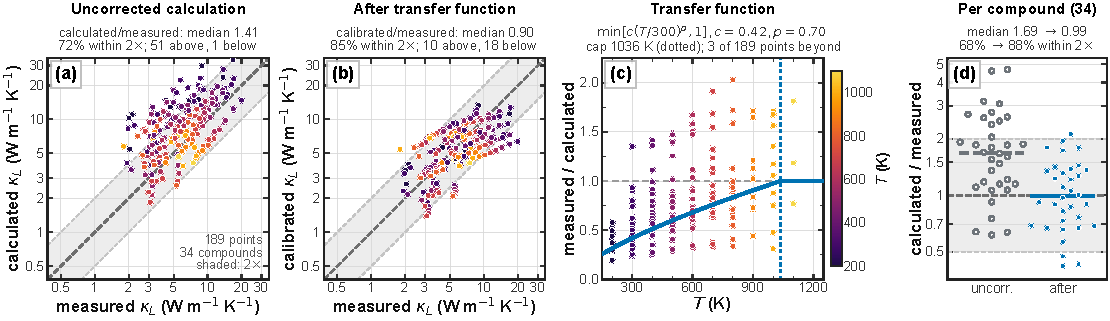
\includegraphics[width=\linewidth]{figures/fig02_offset.pdf}
  \caption{\textbf{Offset between published Boltzmann-transport calculations and measurement, and
  its removal.} (a)~Uncorrected and (b)~calibrated (Eq.~\eqref{eq:transfer}) $\kappa_L$ against
  measurement: \num{189} points, one per compound per \SI{100}{\kelvin} bin, from \num{34}
  in-domain compounds with one reference laboratory each; shaded, within a factor of two; colour,
  temperature; the statistics above (a) and (b) are per point. (c)~Measured/calculated ratio against
  $T$ with the deployed transfer function, $c=\num{0.42}$, $p=\num{0.70}$; dotted, the
  \SI{1036}{\kelvin} cap, beyond which \num{3} of the \num{189} points lie. Points above unity, where
  the calculation already lies below the measurement, are out of reach of a downward correction.
  (d)~Per-compound median calculated/measured ratio before and after correction; bars mark the
  medians (\num{1.69} $\to$ \num{0.99}; within $2\times$, \SI{68}{\percent} $\to$
  \SI{88}{\percent}), the statistics quoted in the text. Calibrated values in (b) and (d) are held
  out (shared constant refitted without each compound's chemistry cluster); the curve in (c) is the
  deployed constant, fitted on all compounds.}
  \label{fig:offset}
\end{figure*}

Correcting each compound with the shared constant refitted without its own chemistry cluster moves
the median ratio from \num{1.69} to \num{0.99} and the fraction of compounds within a factor of two
of measurement from \SI{68}{\percent} to \SI{88}{\percent} (Fig.~\ref{fig:offset}(b) and (d)). The
cap of the shared form binds only above \SI{1036}{\kelvin}, where \num{3} of the \num{189} points
lie (Fig.~\ref{fig:offset}(c)).

\subsection{The transfer function}
\label{sec:transferresults}

\paragraph{The shared constant.} Fitted on the \num{34} compounds of Section~\ref{sec:offset}, the
shared form gives $c=\num{0.42}$ and $p=\num{0.70}$. As Section~\ref{sec:transfer} shows, the
magnitude is stable under removal of any cluster or family and under a bootstrap, whereas the
exponent is not.

\paragraph{One constant per bonding family.}
\label{sec:familycal}
\label{sec:deployed}
A family \emph{member} is a compound with both a usable reference measurement and a
temperature-matched published calculation. Each of the \num{12} families with a member carries its
own constant (Eq.~\eqref{eq:family}), tested leave-one-compound-out because that is the question a
prediction poses: an unmeasured target is predicted with its measured family-mates in hand, and the
family-mates' references are re-chosen inside each fold so that a held-out compound cannot select
them.

Table~\ref{tab:famcal} and Fig.~\ref{fig:family}(a) give the families. Five are validated held out,
all within the \SI{25}{\percent} bar:
\ce{Sb}--\ce{Pt} (\SI{7.4}{\percent}), \ce{Ni}--\ce{Sb} (\SI{16.4}{\percent}), \ce{Fe}--\ce{Sb}
(\SI{17.3}{\percent}), \ce{Sn}--\ce{Pt} (\SI{21.7}{\percent}) and \ce{Co}--\ce{Sb}
(\SI{24.9}{\percent}). In \ce{Sn}--\ce{Pt} the family constant more than halves the shared
constant's error (\SI{50.4}{\percent}), and it is also clearly better in \ce{Sb}--\ce{Pt}
(\SI{30.4}{\percent} with the shared constant) and \ce{Fe}--\ce{Sb} (\SI{28.7}{\percent}). The
\ce{Sb}--\ce{Pt} figure rests on thin data: three of its four
members (\ce{DySbPt}, \ce{LuSbPt}, \ce{TbSbPt}) come from one paper at three temperatures each,
below the four-temperature rule used elsewhere. In \ce{Ni}--\ce{Sb} and \ce{Co}--\ce{Sb} the shared
constant does as well or better on the same compounds (\SI{10.1}{\percent} and
\SI{23.0}{\percent}); the pre-specified rule still gives every family with measured members its own
constant, so the issued \ce{Ni}--\ce{Sb} values carry \num{0.47} rather than the shared \num{0.42}.

\begin{table}[tbp]
  \centering
  \caption{Per-family transfer functions, $\kappa_L^{\mathrm{BTE}}\,c_f\,(T/300)^{0.70}$, with the
  shared exponent. \emph{Held out}: each member predicted from its family-mates alone, with the
  family constant and with the shared constant refitted without it (better in bold); a family is
  \emph{validated} when its held-out error is under \SI{25}{\percent}. \emph{Own paper}: the
  constant fitted on each member's own reference and scored on it, in sample, not a test.
  \textdagger, held-out test not passed; figures in Section~S14 of the Supplementary material, and
  each family's spread of member constants and its publications in Section~S15. The twelfth family,
  \ce{Sb}--\ce{Ir}, has one member that its own constant does not reproduce within the bar even in
  sample; it is listed in Section~S14. Only validated and anchored families issue predictions.}
  \label{tab:famcal}
  \footnotesize
  \setlength{\tabcolsep}{3pt}
  \begin{tabular}{lcccccl}
    \toprule
    & & & \multicolumn{2}{c}{held out (\si{\percent})} & own paper & \\
    \cmidrule(lr){4-5}
    Family & members & $c_f$ & family & shared & (\si{\percent}) & status \\
    \midrule
    \ce{Sb}--\ce{Pt} & 4 & \num{0.61} & \textbf{7.4} & 30.4 & 2.4 & validated \\
    \ce{Ni}--\ce{Sb} & 7 & \num{0.47} & 16.4 & \textbf{10.1} & 4.5 & validated \\
    \ce{Fe}--\ce{Sb} & 3 & \num{0.36} & \textbf{17.3} & 28.7 & 13.9 & validated \\
    \ce{Sn}--\ce{Pt} & 3 & \num{0.89} & \textbf{21.7} & 50.4 & 13.1 & validated \\
    \ce{Co}--\ce{Sb} & 3 & \num{0.42} & 24.9 & \textbf{23.0} & 8.2 & validated \\
    \midrule
    \ce{Bi}--\ce{Pd} & 3 & \num{0.95} & \textdagger & \textdagger & 7.3 & calibrated \\
    \ce{Ni}--\ce{Sn} & 3 & \num{0.32} & \textdagger & \textdagger & 3.0 & calibrated \\
    \ce{Co}--\ce{Sn} & 2 & \num{0.286} & \textdagger & \textdagger & 4.2 & calibrated \\
    \ce{Sb}--\ce{Pd} & 3 & \num{0.24} & \textdagger & \textdagger & 2.8 & calibrated \\
    \midrule
    \ce{Co}--\ce{Bi} & 1 & \num{0.54} & --- & --- & 6.3 & anchored \\
    \ce{Ni}--\ce{Pb} & 1 & \num{0.51} & --- & --- & 5.6 & anchored \\
    \bottomrule
  \end{tabular}
\end{table}

\begin{figure*}[tbp]
  \centering
  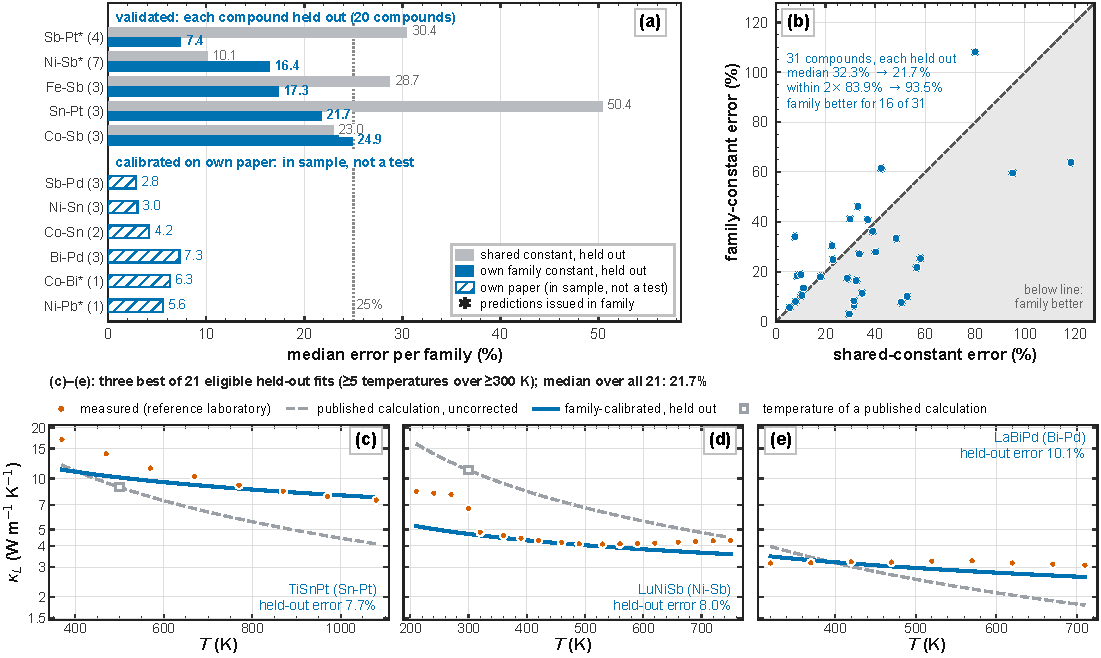
\includegraphics[width=\linewidth]{figures/fig09_family.pdf}
  \caption{\textbf{Per-family calibration on published calculations.} (a)~Median error per bonding
  family ($n$ in brackets; *, families with issued predictions). Validated families (held-out error
  below \SI{25}{\percent}): each member predicted with its family constant fitted without it (blue)
  and with the shared constant refitted without it (grey). Hatched: the four calibrated families and
  the two anchored ones, each constant fitted on its family's own reference papers and scored on
  them, in sample, not a test; held-out figures for the calibrated families are in Section~S14 of
  the Supplementary material. Dotted line, \SI{25}{\percent}. (b)~Shared- against family-constant
  error for all \num{31} held-out compounds; shaded, family constant better (better for \num{16},
  worse for \num{11}, tied for \num{4}; sign test $p=\num{0.44}$). (c)--(e)~$\kappa_L(T)$ for the
  three best of the \num{21} eligible held-out fits (at least five temperatures over at least
  \SI{300}{\kelvin}): illustrations, not a representative sample; the median over all \num{21} is
  \SI{21.7}{\percent}. Points, reference-laboratory measurement; dashed, uncorrected published
  calculation (squares at the calculated temperatures); solid, family-calibrated curve with the
  compound held out. The \ce{LuNiSb} reference joins two instruments: a steady-state measurement up
  to \SI{300}{\kelvin}, which its authors report is affected by radiative losses between
  \SI{200}{\kelvin} and \SI{300}{\kelvin}, and laser flash above~\cite{ciesielski2020thermoelec}.}
  \label{fig:family}
\end{figure*}

Every family reproduces its own reference papers closely: fitted in sample, the median error is
\SIrange{2.4}{13.9}{\percent} across the nine families, and the single-member families fit
\ce{ZrCoBi} (\ce{Co}--\ce{Bi}) to \SI{6.3}{\percent} and \ce{ZrNiPb} (\ce{Ni}--\ce{Pb}) to
\SI{5.6}{\percent}. In four families, \ce{Bi}--\ce{Pd}, \ce{Ni}--\ce{Sn}, \ce{Co}--\ce{Sn} and
\ce{Sb}--\ce{Pd}, the constant fits each paper (\SIrange{2.8}{7.3}{\percent}) but does not transfer
from one member to another within the \SI{25}{\percent} bar, because the members are different
materials as made: a nanostructured against a dense sample, or members measured in different
laboratories, as discussed below. These four are reported as calibrated, not validated; their
held-out figures and the reason in each family are in Section~S14 of the Supplementary material,
and none of them issues a prediction.

\paragraph{Pooled over the held-out compounds.} Thirty-one of the \num{34} compounds belong to a
family with at least one other measured member and can be predicted held out. On the \num{31} such
compounds the family constant gives a median error of \SI{21.7}{\percent}, with \SI{93.5}{\percent}
within a factor of two and \num{17} of the \num{31} under \SI{25}{\percent}. The shared constant,
refitted without each held-out compound and scored on the same \num{31}, gives \SI{32.3}{\percent},
with \SI{83.9}{\percent} within a factor of two. The family constant lowers the median but is not
significantly better compound by compound: it is the better of the two for \num{16} of the
\num{31}, worse for \num{11} and tied for \num{4} (two-sided sign test on the \num{27} untied,
$p=\num{0.44}$). Choosing between the capped and uncapped family forms inside each fold changes
nothing, because the uncapped form is chosen in all \num{31} folds; the capped form throughout gives
\SI{27.0}{\percent}.

Over all \num{34} in-domain compounds with a temperature-matched published calculation, the
uncorrected calculations give \SI{64.1}{\percent} median error, with \SI{70.6}{\percent} within a
factor of two. The shared constant brings that to \SI{31.9}{\percent} and \SI{85.3}{\percent}, and
the family constants to \SI{20.3}{\percent} and \SI{94.1}{\percent}. These figures follow the
protocol of the family test (all matched rows, reference chosen without the family-paper rung, shared
constant refitted without the compound itself), which is why the within-$2\times$ fractions differ
from those of Section~\ref{sec:offset} (per compound against the deployed reference, shared constant
refitted without the chemistry cluster). They also mix the \num{31} held-out compounds with the three
single-member fits, which is why we lead with the held-out comparison.

Figure~\ref{fig:family}(c)--(e) shows what a held-out family fit looks like on individual curves.
Of the \num{21} held-out compounds measured at five or more temperatures over at least
\SI{300}{\kelvin}, it shows the three with the lowest held-out family error, \ce{TiSnPt}
(\ce{Sn}--\ce{Pt}, \SI{7.7}{\percent}), \ce{LuNiSb} (\ce{Ni}--\ce{Sb}, \SI{8.0}{\percent}) and
\ce{LaBiPd} (\ce{Bi}--\ce{Pd}, \SI{10.1}{\percent}), each with its family constant fitted on its own
leave-one-out fold, exactly as the deployed route scores it; they illustrate the method at its best
and are not representative (the median over the \num{21} is \SI{21.7}{\percent}; the full
distribution is Fig.~\ref{fig:family}(b)). Because the family form is uncapped, it can raise $\kappa_L$ above the calculation: with fold constants of \num{0.82} and
\num{0.84} at $p=\num{0.65}$, the factor $c_f(T/300)^{p}$ exceeds one above about \SI{400}{\kelvin}
for \ce{TiSnPt} and \ce{LaBiPd}, so the calibrated curve rises above the uncorrected calculation
there, as the measurements do. This reproduces what the reference measurements report; it is not a
claim that the conductivity exceeds that of the perfect crystal, and every issued prediction lies
below the calculation it calibrates.

\paragraph{What a family constant describes.} Several family constants describe a single kind of
specimen (the publications behind each family are counted in Section~S15 of the Supplementary
material). All three \ce{Sn}--\ce{Pt} references come from one paper, as do three of the four in \ce{Sb}--\ce{Pt}, four of the seven in \ce{Ni}--\ce{Sb} and two
of the three in each of \ce{Bi}--\ce{Pd} and \ce{Sb}--\ce{Pd}; there the held-out test partly
measures one paper's internal consistency rather than transfer between laboratories. Two
\ce{Sb}--\ce{Pd} references are arc-melted ingots whose authors describe the transport as dominated
by grain-boundary and defect scattering~\cite{mukhopadhyay2018multifunct}. The two \ce{Co}--\ce{Sn}
members were measured on very different specimens, \ce{NbCoSn} on a near-fully dense
pellet~\cite{thiem2025thermoelec} and \ce{TaCoSn} on a heavily ball-milled nanocrystalline sample
rich in cobalt interstitials~\cite{li2019ntype}, and a constant fitted on one cannot describe the
other. An anchored family inherits its single member's specimen: \ce{ZrNiPb} was measured only on a
ball-milled sample~\cite{mao2017thermoelec}, so values issued through \ce{Ni}--\ce{Pb} describe a
milled sample, and \ce{ZrCoBi}'s reference is a \SI{98.1}{\percent} dense
pellet~\cite{zhao2018synthesis}, whereas the only other laboratory to measure it reports a value
\num{1.7} times lower near \SI{300}{\kelvin} on a far more heavily milled
specimen~\cite{zhu2018discovery}. The \ce{Co}--\ce{Bi} predictions therefore carry a wider uncertainty
than their conformal band.

\paragraph{The shared constant on families never measured.}
\label{sec:unseenfamily}
For an unmeasured family only the shared constant applies. Withholding each family in turn from the
fit and predicting its members gives, over the \num{34} compounds, a median error of
\SI{33.0}{\percent} with \SI{79.4}{\percent} within a factor of two and \SI{32.4}{\percent} within
\SI{25}{\percent}; per-family medians range from \SI{12.8}{\percent} (\ce{Ni}--\ce{Sb}) to
\SI{116.8}{\percent} (\ce{Sb}--\ce{Pd}). This calibration error travels with every shared-constant
estimate in this paper.

\subsection{The regression model reproduces published calculations}
\label{sec:mlrepro}

Where no calculation is published, the model supplies one. Scored against the published full
calculations of the \num{230} $\mathrm{VEC}=18$ half Heuslers, each predicted with its X-site
chemistry cluster withheld from training (\num{27} clusters), the median error is
\SI{21.9}{\percent} (one seed, the reference seed), with \SI{88.3}{\percent} within a factor of two
and a median ratio of \num{0.87} (Fig.~\ref{fig:modelblind}(a)). This describes only the step
from structure to calculation; the end-to-end test below already contains it, so the two errors are
never stacked. Three of the four regressors of Table~\ref{tab:models} reach nearly the same
accuracy.

\begin{figure*}[tbp]
  \centering
  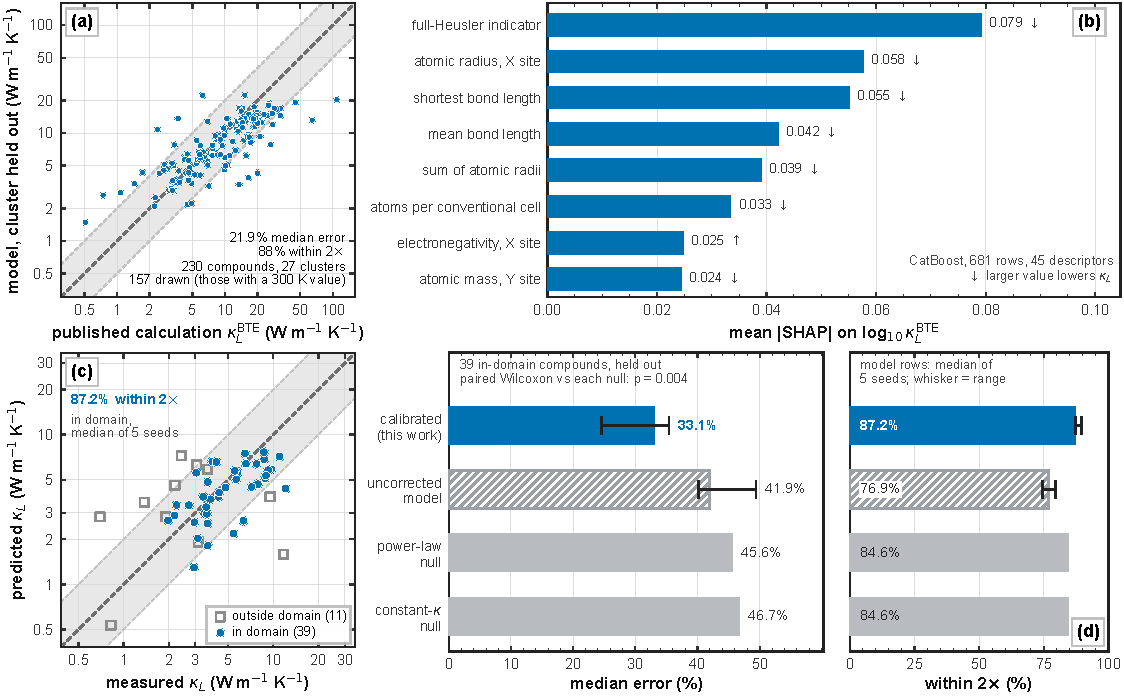
\includegraphics[width=\linewidth]{figures/fig15_model_blind.pdf}
  \caption{\textbf{From crystal structure to measured $\kappa_L$.} (a)~Model against the published
  full Boltzmann-transport calculation, each compound's X-site chemistry cluster removed from
  training: \SI{21.9}{\percent} median error and \SI{88.3}{\percent} within $2\times$ over
  \num{230} compounds (single seed; per compound over all calculated temperatures); those with a
  \SI{300}{\kelvin} value are drawn. Shaded, within a factor of two. (b)~The eight descriptors with
  the largest mean $|\textsc{shap}|$ attribution to $\log_{10}\kappa_L^{\mathrm{BTE}}$; arrows give
  the direction of the effect of a larger value. The training pool includes full Heuslers, so the
  full-Heusler indicator, which ranks first, partly reflects the make-up of the pool; the full
  attribution is in Section~S7 of the Supplementary material. (c)~Blind test against measurement, the chemistry
  cluster held out of both the model and the transfer function: filled, the \num{39} compounds
  inside the domain of applicability; open, the \num{11} outside it. Points are from the reference
  seed; the printed within-$2\times$ fraction is the five-seed median. (d)~Median error and fraction
  within $2\times$ on the \num{39} in-domain compounds for the calibrated route, the uncorrected
  model, and the power-law and constant-$\kappa$ nulls, both nulls fitted with the chemistry held
  out; model rows are the median of five seeds with the seed range as whiskers, the nulls are
  seed-free; paired Wilcoxon $p=\num{0.004}$ against each null.}
  \label{fig:modelblind}
\end{figure*}

\subsection{What the model has learned}
\label{sec:shap}

We decompose the reference-seed model, fitted on all \num{681} training rows, with \textsc{shap}
(SHapley Additive exPlanations)~\cite{lundberg2017a}, which assigns each descriptor an additive
contribution to each prediction; on the $\log_{10}$ target a contribution of $+0.1$ multiplies the
predicted calculation by about \num{1.26}. Figure~\ref{fig:modelblind}(b) shows the eight
descriptors with the largest mean absolute contribution, and Section~S7 of the Supplementary
material the twelve largest with the contribution to every training row; signs are read from the
correlation between a descriptor's value and its contribution (in parentheses: mean
$|\textsc{shap}|$, then that correlation). The full-Heusler flag leads (\num{0.079}, \num{-0.99}): a full Heusler is predicted to conduct less. Size
and bond length come next: the X-site radius (\num{0.058}), the shortest bond (\num{0.055}), the
mean bond length (\num{0.042}) and the sum of radii (\num{0.039}) all lower the prediction as they
grow (correlations \num{-0.71} to \num{-0.93}), as do more atoms per conventional cell (\num{0.033},
\num{-0.98}) and a heavier Y site (\num{0.024}, \num{-0.82}). The X-site electronegativity
(\num{0.025}, \num{+0.43}) and $1/T$ (\num{0.018}, \num{+0.90}) raise it. This is consistent with
phonon physics: heavier atoms, longer and softer bonds and more atoms per cell lower a lattice's
conductivity, and Umklapp scattering weakens as temperature falls. Consistency does not show that the
model has learned that physics.

Three cautions apply. The attribution explains the model of the \emph{calculation}, not of a
measurement, which also depends on the specimen. Correlated descriptors share attribution (the sum
of radii and the mean radius, the shortest and mean bond lengths, atoms per cell and the
full-Heusler flag; correlation map in Section~S7 of the Supplementary material), so the ranking describes groups
of descriptors more reliably than individual ones. And the full-Heusler flag partly reflects the
make-up of the pool, whose full-Heusler labels include semi-empirical estimates; it shifts all
half-Heusler predictions together and does not reorder them.

\subsection{End to end: from crystal structure to measurement}
\label{sec:blind}

This is the paper's central accuracy figure: how close the full chain, model plus shared transfer
function, comes to measurement for a compound whose chemistry was withheld from every fitted step.
We score the \num{39} in-domain half Heuslers, each against its single reference laboratory with its
X-site chemistry cluster removed from both the model's training and the fit of the shared constant.

The calibrated prediction has a median error of \SI{33.1}{\percent} and places \SI{87.2}{\percent} of
compounds within a factor of two of measurement (Fig.~\ref{fig:modelblind}(c) and (d)), both
medians over five model seeds; the full table, with the fraction within \SI{30}{\percent} and the
bias of every route, is in Section~S16 of the Supplementary material. Across seeds the median error
ranges from \SI{24.6}{\percent} to \SI{35.4}{\percent}, so it should be read as roughly one third; the within-$2\times$ fraction (\SIrange{87.2}{89.7}{\percent})
and the rank correlation are stable by comparison. Without the correction the same model output gives
\SI{41.9}{\percent} and \SI{76.9}{\percent}; the correction moves the median ratio of predicted to
measured conductivity from \num{1.40} to \num{0.90}. The \num{39} include \ce{YNiBi}, whose every
measured curve fails the curve-shape test (its lattice conductivity rises with temperature) and which
keeps its measurement, ranked last, so that the scored population does not depend on that test.
Without \ce{YNiBi} the headline is \SI{33.1}{\percent} (seed range \SIrange{24.6}{35.5}{\percent})
over \num{38} compounds, with \SI{86.8}{\percent} within a factor of two, and the paired comparison
with the null baselines gives $p=\num{0.005}$ and $p=\num{0.006}$ (medians over seeds).

\paragraph{Against compound-blind baselines.}
\label{sec:vsnulls}
The constant and power-law null baselines, refitted with the same chemistry held out and scored
against the same references, give \SI{46.7}{\percent} and \SI{45.6}{\percent} median error, against
our \SI{33.1}{\percent} (Fig.~\ref{fig:modelblind}(d)). A paired Wilcoxon signed-rank test on the per-compound
errors gives $p=\num{0.004}$ against each null at the median over seeds, and $p$ is below \num{0.05}
against both on every seed. Compounds of one chemistry cluster share a model fold and often a
laboratory, so we repeat the test counting each of the \num{18} clusters once, by its median error:
the cluster-level Wilcoxon test gives $p<0.05$ on every seed against both nulls (largest \num{0.039}
against the constant and \num{0.048} against the power law), but the cluster-level sign test is not
significant on every seed ($p$ from \num{0.0013} to \num{0.48} against the constant and from
\num{0.0013} to \num{0.096} against the power law). With two nulls, five seeds and no correction for
multiple comparisons, the cluster-level evidence is marginal. Both nulls place slightly fewer
compounds within a factor of two (\SI{84.6}{\percent}), so the gain lies in the typical error rather
than in the tail.

\paragraph{Without the domain screens.} Over all \num{50} measured half Heuslers the same protocol
gives \SI{38.6}{\percent} median error (seed range \SIrange{36.8}{38.8}{\percent}), with
\SI{78.9}{\percent} within a factor of two, against \SI{47.3}{\percent} uncorrected. The comparison
with the nulls holds, more weakly: at the reference seed, over the \num{50} compounds (\num{21}
clusters), the model route gives \SI{36.4}{\percent} against \SI{48.7}{\percent} for the constant null
and \SI{48.2}{\percent} for the power law (paired Wilcoxon $p=\num{0.035}$ and $p=\num{0.033}$).

\paragraph{Outside the domain.}
\label{sec:failure}
The eleven compounds the screens exclude (\ce{AlNiSb}, \ce{BaAgSb}, \ce{LaSbPd}, \ce{LiAlGe},
\ce{LiAlSi}, \ce{LiZnSb}, \ce{MgAgSb}, \ce{MgNiSb}, \ce{NbCoSb}, \ce{VCoSb}, \ce{VNiSn}) behave as a
separate population: at the reference seed their median error is \SI{86.4}{\percent}, against
\SI{31.7}{\percent} inside the domain (Mann--Whitney $p=\num{5.1e-5}$), with \SI{36.4}{\percent}
within a factor of two and a median bias of \num{1.74} (open squares in
Fig.~\ref{fig:modelblind}(c)).

\paragraph{Ranking, temperature term and semi-empirical estimates.} Spearman's $\rho$ between
predicted and measured conductivity is \num{0.662} (seed range \numrange{0.642}{0.699}); at a fixed
temperature this ordering comes from the model, and the correction adds the temperature term and the
absolute scale of a screening threshold. Without the temperature term
($\kappa_L^{\mathrm{exp}} = c\,\kappa_L^{\mathrm{BTE}}$) the error rises to \SI{38.5}{\percent} and
the within-$2\times$ fraction falls to \SI{82.1}{\percent}; at the reference seed (one seed) the
paired difference is \num{7.7} pp (Wilcoxon $p=\num{0.0143}$), the two-parameter form closer for
\SI{61.5}{\percent} of compounds. Published Slack~\cite{slack1979the} and Debye--Callaway estimates,
on the \num{22} in-domain compounds that have one, give \SI{91.6}{\percent} with
\SI{54.5}{\percent} within a factor of two and a bias of \num{1.92}; they are published values with
no holdout and are not paired with the blind-test set.

\paragraph{Where the error falls, and a family-informed baseline.}
\label{sec:familynull}
At the reference seed the worst families on the model route are \ce{Co}--\ce{Sn}
(\SI{59.4}{\percent}) and \ce{Ni}--\ce{Sn} (\SI{55.4}{\percent}), three compounds each, while
\ce{Ni}--\ce{Sb} (eight compounds: the seven members of Table~\ref{tab:famcal} and \ce{YbNiSb}) is at
\SI{13.7}{\percent}; this grouping is descriptive, since the holdout unit is the X site. A stronger
baseline fits a power law to the measured $\kappa(T)$ of the held-out compound's own family, with no
calculation. On the \num{34} in-domain compounds where it is defined (the \num{39} minus \ce{AlVNi},
\ce{YNiBi}, \ce{ZrCoBi}, \ce{ZrNiPb} and \ce{ZrSbIr}; not the \num{34} of the published route), it
gives \SI{25.4}{\percent} against \SI{31.6}{\percent} for the model route at the reference seed, with
neither significantly better (paired Wilcoxon $p=\num{0.99}$; model closer for \SI{50.0}{\percent}).
Where a family has been measured we do not beat it on absolute accuracy, but it cannot order
compounds within a family or say anything where no member is measured. For scale, calibrating a
published calculation with the shared constant gives \SI{32.3}{\percent} on the \num{31} compounds of
the family test, comparable to the model route's \SI{33.1}{\percent} on a different population.

\subsection{A published machine-learned model}
\label{sec:sdnnff}

Elemental-SDNNFF obtains $\kappa_L$ through the Boltzmann transport equation on a neural-network
force field~\cite{rodriguez2023millionsca}, so its values are tier~2 and were never labels; the same
paper's ShengBTE values are tier~1 and enter the published-calculation median for \num{6} of the
\num{18} compounds below (\ce{NbFeSb}, \ce{TaFeSb}, \ce{TiNiSn}, \ce{VFeSb}, \ce{ZrCoSb},
\ce{ZrNiSn}). On those \num{18} in-domain compounds SDNNFF reproduces the published calculations at
\SI{300}{\kelvin} to a median \SI{18.8}{\percent} (ratio \num{0.99}). Against measurement, on the
\num{21} in-domain compounds it covers, it lies a median factor of \num{2.01} above the reference
(\SI{101.4}{\percent} median error, \SI{42.9}{\percent} within a factor of two), and the published
calculations lie a factor of \num{1.99} above measurement on their \num{18} (a different set from
Section~\ref{sec:offset}, at \SI{300}{\kelvin} only, for matching windows from \SI{\pm 25}{\kelvin}
to \SI{\pm 100}{\kelvin}): the offset arrives intact at the end of a screening pipeline. The shared
constant, refitted without each compound's chemistry cluster, brings the SDNNFF values to
\SI{36.8}{\percent} with \SI{76.2}{\percent} within a factor of two (paired Wilcoxon $p=\num{0.0033}$),
so the correction transfers to an independent source of calculations. Our model route gives
\SI{44.7}{\percent} on the same \num{21} (reference seed, \SI{71.4}{\percent} within a factor of two),
closer to measurement than raw SDNNFF for \num{16} of the \num{21} (paired Wilcoxon
$p=\num{0.0055}$) but not as close as calibrated SDNNFF, in a comparison tilted towards SDNNFF, whose
values are given no holdout.

\subsection{Predictions for unmeasured compounds}
\label{sec:screening}
\label{sec:issued}

We apply the family route to half Heuslers that have a published transport calculation but no
measurement. A candidate is issued only if it meets every condition below:
\begin{enumerate}
  \item \textbf{Inside the domain of applicability} (Section~\ref{sec:domain}), with no radioactive
        and no valence-fluctuating element.
  \item \textbf{A bonding family whose constant has been checked}: \emph{validated} (held-out error
        under \SI{25}{\percent}) or \emph{anchored} on a single member whose in-sample fit is under
        the same bar, an anchored prediction carrying that label (Table~\ref{tab:famcal}).
  \item \textbf{A full transport calculation}, independent calculations agreeing within a factor of
        two at the quoted temperature.
  \item \textbf{Inside, or only marginally outside, the family's measured range.} A value beyond the
        family's measured span by less than a factor of \num{1.33}, the median disagreement between
        laboratories, is issued with a \emph{marginal} label; a value further outside is flagged.
\end{enumerate}

Ten compounds meet every condition (Table~\ref{tab:predictions}, Fig.~\ref{fig:predictions}). Three
lie inside the span of a validated family: \ce{TmSbPt} in \ce{Sb}--\ce{Pt}, and \ce{GdNiSb} and
\ce{TbNiSb} in \ce{Ni}--\ce{Sb}, each differing from the measured members only on the rare-earth
site. Three are marginal extrapolations in \ce{Sb}--\ce{Pt}: \ce{ErSbPt} and \ce{HoSbPt} a factor of
\num{1.15} and \num{1.12} above the family's span, and \ce{GdSbPt} \num{1.03} below it. As a check,
the \num{6} measured compounds lying this close outside their family-mates' span were predicted held
out to a median of \SI{17.4}{\percent}, \num{3} of them under \SI{25}{\percent}, against
\SI{18.8}{\percent} for the \num{19} inside it (two-sided Mann--Whitney $p=\num{0.51}$). Four issue
through anchored families: \ce{HfCoBi} and \ce{TiCoBi} through \ce{Co}--\ce{Bi}, and \ce{HfNiPb} and
\ce{TiNiPb} through \ce{Ni}--\ce{Pb}. Four of the ten issue through \ce{Sb}--\ce{Pt}, whose
validation rests mainly on one paper (Section~\ref{sec:familycal}). \ce{TiCoBi}, \ce{HfNiPb} and \ce{TiNiPb} are quoted at
\SI{500}{\kelvin}, the temperature of their only uncontested calculation (for \ce{TiNiPb}, the two
\SI{300}{\kelvin} calculations disagree \num{5.6}-fold).

\begin{table*}[tbp]
  \centering
  \caption{The ten issued predictions of lattice thermal conductivity for half Heuslers with a
  published transport calculation and no measurement, each through its own family's constant
  (Table~\ref{tab:famcal}). $T$ is \SI{300}{\kelvin}, or \SI{500}{\kelvin} where that is the
  temperature of the only uncontested calculation; $\kappa_L^{\mathrm{BTE}}$ is the median published
  calculation at $T$. The \SI{90}{\percent} intervals are conformal at the quoted temperature; the
  \SI{50}{\percent} intervals, a factor of \num{1.62} (\SI{300}{\kelvin}) or \num{1.38}
  (\SI{500}{\kelvin}) either way, are drawn in Fig.~\ref{fig:predictions}. For the anchored families
  their coverage is not validated. Span places the value relative to the range of the family's
  compounds measured near \SI{300}{\kelvin}: inside it, or beyond it by the factor shown (marginal).
  An anchored family defines no span.}
  \label{tab:predictions}
  \small
  \begin{tabular}{llccccc}
    \toprule
    Compound & Family (basis, $c_f$) & $T$ & $\kappa_L^{\mathrm{BTE}}$ & \textbf{Predicted} &
      \SI{90}{\percent} interval & span \\
    & & (\si{\kelvin}) & \multicolumn{3}{c}{(\si{\watt\per\meter\per\kelvin})} & \\
    \midrule
    \ce{TmSbPt} & \ce{Sb}--\ce{Pt} (validated, \num{0.61}) & 300 & 5.86 & \textbf{3.57} & 1.25--10.17 & inside \\
    \ce{GdNiSb} & \ce{Ni}--\ce{Sb} (validated, \num{0.47}) & 300 & 8.38 & \textbf{3.94} & 1.38--11.23 & inside \\
    \ce{TbNiSb} & \ce{Ni}--\ce{Sb} (validated, \num{0.47}) & 300 & 9.59 & \textbf{4.51} & 1.58--12.85 & inside \\
    \ce{ErSbPt} & \ce{Sb}--\ce{Pt} (validated, \num{0.61}) & 300 & 7.18 & \textbf{4.38} & 1.54--12.48 & \num{1.15} above \\
    \ce{HoSbPt} & \ce{Sb}--\ce{Pt} (validated, \num{0.61}) & 300 & 7.00 & \textbf{4.27} & 1.50--12.17 & \num{1.12} above \\
    \ce{GdSbPt} & \ce{Sb}--\ce{Pt} (validated, \num{0.61}) & 300 & 3.34 & \textbf{2.04} & 0.72--5.81 & \num{1.03} below \\
    \midrule
    \ce{HfCoBi} & \ce{Co}--\ce{Bi} (anchored, \num{0.54}) & 300 & 18.60 & \textbf{10.04} & 3.52--28.61 & --- \\
    \ce{TiCoBi} & \ce{Co}--\ce{Bi} (anchored, \num{0.54}) & 500 & 19.10 & \textbf{14.75} & 7.80--27.88 & --- \\
    \ce{HfNiPb} & \ce{Ni}--\ce{Pb} (anchored, \num{0.51}) & 500 & 9.96 & \textbf{7.26} & 3.84--13.72 & --- \\
    \ce{TiNiPb} & \ce{Ni}--\ce{Pb} (anchored, \num{0.51}) & 500 & 13.91 & \textbf{10.14} & 5.37--19.16 & --- \\
    \bottomrule
  \end{tabular}
\end{table*}

% [!t]: at [tbp] the figure plus caption exceeds \topfraction and LaTeX set it alone on a float
% column with half the column empty; ! lifts the fraction limits so it heads the column instead.
\begin{figure}[!t]
  \centering
  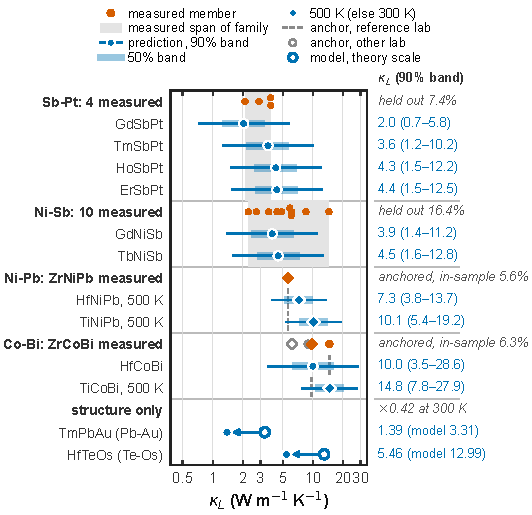
\includegraphics[width=\columnwidth]{figures/fig05_predictions.pdf}
  \caption{\textbf{Issued predictions beside the measurements that license them.} Each row is one
  issued compound at its quoted temperature (diamonds, \SI{500}{\kelvin}; otherwise
  \SI{300}{\kelvin}), with its \SI{50}{\percent} (thick) and \SI{90}{\percent} (thin) conformal
  intervals. Validated families: orange dots, measured members near \SI{300}{\kelvin}; grey band, the
  span they define. A family's measured count includes compounds without a published calculation,
  so it can exceed its member count in Table~\ref{tab:famcal}. Anchored families (one measured
  member): orange marker and dashed line, that member's reference-laboratory value at the quoted
  temperature; open grey marker, a second laboratory's. Bottom: the two structure-only predictions,
  the model's calculation-scale value (open) and the value after the shared transfer function
  (filled). The model error (Fig.~\ref{fig:modelblind}(a)) and the transfer-function error
  (Section~\ref{sec:unseenfamily}) are reported separately, not combined.}
  \label{fig:predictions}
\end{figure}

The conformal bands (Section~\ref{sec:intervals}) are a factor of \num{1.62} and \num{2.85} at
\SI{300}{\kelvin} (per-seed ranges \numrange{1.61}{1.67} and \numrange{2.70}{3.02}) and \num{1.38}
and \num{1.89} at \SI{500}{\kelvin} (\numrange{1.31}{1.41} and \numrange{1.86}{1.94}) for the
\SI{50}{\percent} and \SI{90}{\percent} levels. The calculations being calibrated come from published
high-throughput
studies~\cite{li2025highthroug,ohnishi2026database,miyazaki2021machine,carrete2014finding,trans2022lattice},
most from one~\cite{miyazaki2021machine}. Seven of the ten rest on a single published calculation at
the quoted temperature. Independent calculations of the same half Heusler disagree by a median
factor of \num{1.37}, and the band describes the error of the transfer function, not the spread among
its inputs, so where only one calculation exists the band is a lower bound on the uncertainty. Nine
of the ten rest on a calculation at a single temperature (\ce{HfCoBi} on two), so no other
temperature is quoted. \ce{GdNiSb} also carries a structural caveat the databases do not record: it
has been reported in a high-temperature \ce{AlB2}-type hexagonal form beside the low-temperature
\ce{MgAgAs}-type cubic one~\cite{skolozdra1997magnetic}, and the prediction is for the cubic phase.

\subsection{Flagged compounds, and what would release them}
\label{sec:refusals}

Fifteen compounds carry a calibrated value but are declined (\emph{flagged}); Section~S13 of the
Supplementary material tabulates each with the check it fails and draws every status on one axis. Nine are
\ce{Bi}--\ce{Pd} compounds, a family calibrated on its papers but not validated held out; seven also
lie a factor of \numrange{1.36}{1.86} above the \SIrange{3.2}{3.5}{\watt\per\meter\per\kelvin} span
of the two \ce{Bi}--\ce{Pd} compounds measured near room temperature. \ce{TmSbPd} and \ce{DySbPd}
belong to \ce{Sb}--\ce{Pd}, likewise calibrated but not validated, and \ce{DySbPd} is also
polymorphic. \ce{LaSbPt} and \ce{ScSbPt} are clear extrapolations in a validated family, a factor of
\num{2.00} below the measured \ce{Sb}--\ce{Pt} floor and \num{1.97} above its ceiling. \ce{HfSbIr}
and \ce{TiSbIr} belong to \ce{Sb}--\ce{Ir}, whose single measured member its own constant does not
reproduce within the bar. The range gate is a conservative
choice rather than a validated filter: the two held-out compounds that lay further outside their
family's span were predicted to a median of \SI{18.4}{\percent}, but two cases cannot justify issuing
clear extrapolations.

Ten further estimates, in \ce{Ni}--\ce{Bi}, are conditional. The family's only measured member,
\ce{YNiBi}, reports a lattice conductivity that rises with temperature, which its authors attribute
to a bipolar contribution~\cite{li2015synthesis}, so the family cannot be calibrated. On the shared
constant the ten lie at \SIrange{2.21}{4.95}{\watt\per\meter\per\kelvin} at \SI{300}{\kelvin};
Section~S1 of the Supplementary material lists them with the two measurements that would release
them, and one of them,
\ce{SmNiBi}, is also flagged because samarium's valence is not fixed. Across the three statuses the
conformal band has the same relative width; what changes is the evidence behind the value, not its
stated precision.

Not every gap can be closed by a measurement. The cobalt arsenides \ce{XCoAs} (X = Ti, Zr, Hf) have
published calculations but no measured family member, and the two synthesised, \ce{ZrCoAs} and
\ce{HfCoAs}, form the orthorhombic \ce{Co2Si} type~\cite{kleinke1998crystal}. The polymorph screen
catches \ce{HfCoAs}, which has an orthorhombic record (space group 62), but not \ce{ZrCoAs} or
\ce{TiCoAs}, whose records carry only the cubic cell.

\subsection{Predictions from crystal structure alone}
\label{sec:structonly}

For compounds with no published lattice-thermal-conductivity calculation, the model supplies
$\kappa_L^{\mathrm{BTE}}$ and the shared constant maps it onto the experimental scale. Each value
carries two separately validated errors, which we state side by side rather than combine: the model
step, \SI{21.9}{\percent} median error (one seed) with \SI{88.3}{\percent} within a factor of two
against published calculations (Section~\ref{sec:mlrepro}), and the calibration step, the shared
constant on a family never measured, \SI{33.0}{\percent} median with \SI{79.4}{\percent} within a
factor of two (Section~\ref{sec:unseenfamily}). Two compounds are graded strong on the evidence for
their model step; Fig.~\ref{fig:predictions} (bottom) gives both values for each. No conformal band is
given, because its coverage is not validated for a family never measured.

\ce{TmPbAu} (\ce{Pb}--\ce{Au}; OQMD cubic cell, $a=\SI{6.782}{\angstrom}$, the lowest-energy
ordering). The six \ce{Pb}--\ce{Au} half Heuslers with published calculations are reproduced held out
to between \SI{1}{\percent} and \SI{13}{\percent} (median \SI{8.6}{\percent}), and the seeds agree
within a factor of \num{1.11}. The model gives \SI{3.31}{\watt\per\meter\per\kelvin} and the shared
constant ($c=\num{0.42}$) \SI{1.39}{\watt\per\meter\per\kelvin} at \SI{300}{\kelvin}. We found no
published report of \ce{TmPbAu}; a family neighbour, \ce{TbAuPb}, has been grown as single crystals in
the cubic half-Heusler structure~\cite{agarwal2026thermodyna}.

\ce{HfTeOs} (\ce{Te}--\ce{Os}; AFLOW cubic cell, $a=\SI{6.33}{\angstrom}$, the lowest-energy
ordering). The strong grade rests on one member, \ce{TiTeOs}, reproduced to \SI{0.5}{\percent} held
out; the seeds spread by a factor of \num{1.23}. The model gives \SI{12.99}{\watt\per\meter\per\kelvin}
and the shared constant \SI{5.46}{\watt\per\meter\per\kelvin}. The SDNNFF value for the twin
\ce{ZrTeOs}~\cite{rodriguez2023millionsca}, carried to hafnium by the twin ratio of the Extended
Methods, gives \SI{14.06}{\watt\per\meter\per\kelvin}, of which the model value is \num{0.92}; that
ratio was validated on calculated pairs (\SI{12.2}{\percent} against \SI{9.8}{\percent} for the
model), not on a machine-learned input, so the cross-check is weaker than its validation suggests. We
found no published report of \ce{HfTeOs}.

The search also found further compounds with no published $\kappa_L$ and a group with only a
machine-learned value from a published screen; Section~S11 of the Supplementary material reports
them, together with two compounds in calibrated families that are flagged.

\subsection{Limits of the method}
\label{sec:limitations}

\textbf{Temperature dependence is not predicted.} One exponent serves every compound and it is
poorly determined (bootstrap range \numrange{0.45}{1.15} against \numrange{0.35}{0.55} for $c$;
Section~\ref{sec:transfer}), and the training labels sit mostly at \SI{300}{\kelvin}. Every value in
this paper is a value at a stated temperature, and none should be read as a curve.

\textbf{One reference laboratory per compound.} Laboratories measuring the same in-domain compound
disagree by a median factor of \num{1.33} over all pairs of measurements (\num{1.36} taking each
compound's median), so an error of a third is close to the reproducibility of the field, and per-family
errors may fall below that level partly because each compound is scored against one chosen reference.

\textbf{The compounds are not independent.} They share chemistry clusters, bonding families and, in
places, a laboratory, so the effective sample is smaller than \num{39}; the cluster-level tests
address the first, not the shared laboratories.

\textbf{A family constant is interpolation within the family}, and in several families the
family-mates are one paper's specimens. A family nobody has measured receives only the shared
constant, with its \SI{33.0}{\percent} median error, and the capped shared correction cannot raise a
calculation that already lies below its measurement.

\textbf{The issued values rest on few calculations.} Seven of the ten rest on a single published
calculation at the quoted temperature, and most on one study. A systematic error there would pass
undiluted into those values; a transfer function calibrates the scale of a calculation, not its
correctness.

\textbf{Training is restricted to full calculations}, leaving \num{284} half Heuslers to learn from.
The pool still contains two compounds that are not Heuslers, \ce{BaBrCl} and \ce{NaAgO}, and
\num{81} rows without bond descriptors; the model handles a missing descriptor natively, and the
effect on the reported accuracy is expected to be small.

\textbf{Structure-only values carry two errors and assume a structure}: neither compound has, as far
as we could find, been synthesised, so each value is conditional on the cubic phase forming.

\textbf{Alternatives tested.} A correction without the temperature term (Section~\ref{sec:blind}), a
capped family form, a two-stage (hurdle) model, a magnitude-dependent calibration term, and training
on experimental or doped-composition values were tested and not adopted, because they did not
improve held-out accuracy consistently.
